\documentclass{article}
\usepackage[preprint]{neurips_2023}
\usepackage[utf8]{inputenc}
\usepackage[T1]{fontenc}
\usepackage{hyperref}
\usepackage{url}
\usepackage{booktabs}
\usepackage{amsmath,amsfonts}
\usepackage{microtype}
\usepackage{xcolor}
\usepackage{graphicx}
\usepackage{array}
\usepackage{enumitem}
\usepackage{pgfplots}
\pgfplotsset{compat=1.18}
\usepgfplotslibrary{groupplots}
\setlist{nosep,leftmargin=*}
\hypersetup{colorlinks=true,linkcolor=blue!50!black,citecolor=blue!50!black,urlcolor=blue!50!black}

\title{Do Monitors of Latent Thoughts Read What the Model Uses?\\[3pt]\large A causal audit of continuous-thought reasoners, and of a published latent safety monitor}

\author{%
  Muhammad Jon Raza
  \And
  Zain Ahmed
}

\begin{document}
\maketitle

\begin{abstract}
Several recent language models reason in a short sequence of continuous vectors (``latent thoughts'') rather than in text, and the proposed way to oversee them is a linear probe on those vectors. A probe establishes what a thought \emph{contains}. It does not establish that the model \emph{uses} what it contains. We ask whether the two come apart, and we answer with interventions only, on released checkpoints, with every prediction registered before each run. First, a one-command audit measures for each thought whether it carries a value into the answer, whether the model needs it, and whether a probe's reading of it is confirmed by behaviour. On eight checkpoints (CODI and SIM-CoT at 124M to 8B, Coconut, and two models trained on a logic task) the thoughts that read best are routinely the ones the model never acts on; below 8B the readable slot holds a stale copy of a value an earlier thought computed and handed on. Second, we retrain the model of a published latent safety monitor \citep{ramjee2026ulterior} from its authors' recipe, together with an inert-trigger control the original lacked. The probe transfers at 1.000 on the backdoored model and 0.53 on the control, yet swapping, removing or editing the probed thoughts moves the model's behaviour by less than 0.005 against a 0.19 effect: the probe reads a training-installed copy of the trigger, and the backdoor is decided in the memory of the ordinary prompt words. Third, a model retrained so that its answer can only read its thoughts makes them load-bearing, and there steering along the direction the behaviour moves on removes the backdoor's effect, while steering along the direction the probe reads moves nothing on either model. Two legitimate uses of a thought monitor survive: a tamper on the carrying thought leaves a seam the next position does not follow (AUROC 0.92 to 0.98), and routing the least confident quarter of problems to the model's own written solution gains 3.7, 7.5 and 10.2 points at 1B, 3B and 8B. Nothing read from the thoughts improves either. All 39 runs reproduce byte for byte.
\end{abstract}

\section{Introduction}

A model that reasons in text can be read; its steps are tokens. Coconut \citep{hao2024coconut}, CODI \citep{shen2025codi} and SIM-CoT \citep{wei2026simcot} move the steps into a handful of continuous vectors that no reader can decode directly, and the field's response has been to train a probe on the vectors and treat its accuracy as monitorability. \citet{ramjee2026ulterior} go furthest: they plant a dual-trigger backdoor in a Coconut-style model, show that a probe on the early thoughts detects the armed state at 89\%, and recommend monitoring those positions.

That recommendation rests on an assumption the probe cannot test. A probe shows that a quantity is linearly present in a vector. Whether the model goes on to use that quantity, and whether the answer would differ without it, are causal questions, and prior work on these models has raised them without settling them on released weights. \citet{cywinski2025} patched single thoughts of a self-trained CODI on templated problems; \citet{dilgren2026interpretable} showed that on logic tasks the thoughts can be dropped at no cost; \citet{aswal2026observable} showed that decodable patterns appear in controls without recurrence; \citet{li2026dynamics} measured flip rates under step-wise zeroing. None asked, for a given thought, whether what a probe reads from it is what the model acts on, and none applied that test to a monitor that someone has proposed to deploy.

This paper narrows the question to one distinction, \emph{readable} against \emph{used}, and decides it three ways. We run no training on any released model; we change what is inside the model while it runs and watch the answer. Every run was preregistered in a public ledger with its predictions, scored afterwards, and reproduced on a second account.

The closing tests are these. (i) On eight released checkpoints, does a thought that a probe reads well carry a value into the answer, and does the model need it? We find that one or two of six do, that the model often does not need even those, and that the most readable thought is frequently a stale copy of a value handed on earlier. (ii) On the model of a published safety monitor, retrained from its authors' recipe with a control they did not run, does the probe read the cause of the behaviour or a copy of its trigger? We find a copy: perfect transfer, no causal effect, and the behaviour decided in the prompt's own memory. (iii) Can the thoughts be steered, and does that depend on whether the model uses them? We find that it depends on exactly that, by building a model whose answer can read only its thoughts and repeating the audit on it. Two uses of a thought monitor remain, tamper evidence and confidence routing, and we measure both.

\section{Related work}

\paragraph{Continuous-thought models.} Coconut feeds the last hidden state back as the next input embedding and replaces reasoning steps by a curriculum. CODI distils an explicit-chain teacher into six thoughts through a projector. SIM-CoT adds step-level supervision. We audit released CODI and SIM-CoT checkpoints, a third-party Coconut retrain, and the ProsQA checkpoints of \citet{dilgren2026interpretable}.

\paragraph{Causal analyses of latent thoughts.} \citet{cywinski2025} found, on twenty three-step templates, that the third and fifth latents of CODI-1B store the two step values and that the last two can be replaced at no cost; our carriers and inert terminal confirm that placement on natural data. \citet{li2026dynamics} zero single steps and report flip rates; \citet{dilgren2026interpretable} mean-ablate all latents and decode intermediate results from the top-1 integer token; \citet{jin2026final} find accuracy and counterfactual responsiveness diverging over training. None separates a thought's transport from its necessity, nor a probe's reading from its confirmation.

\paragraph{Editing thoughts.} \citet{chang2026unlocking} edit an early cached thought at decoding time and transplant latent sequences between instances, gaining 0.4 to 1.8 points without a value-matched donor or a control. \citet{huang2026steering} find that synthetic steering does not reach the output. Our write is value-matched, controlled, and reported with its harm and its ceiling.

\paragraph{Monitors.} \citet{ramjee2026ulterior} is the monitor we test. That decodability is not causality is established in principle \citep{openproblems2025,decodability2026}; we measure the gap per thought on latent reasoners and on a proposed monitor.

\section{Instruments}\label{sec:instruments}

\paragraph{Two routes.} A thought at slot $s$ reaches the answer by its output state, projected into slot $s{+}1$'s input, and by the keys and values it writes into the cache that every later position attends to. Hooks edit either route on the released decoding path; feeding a thought its own recorded state or cache back is the identity, which is checked before every run.

\paragraph{Twins and transport.} Swapping an unrelated problem's thought breaks answers, and breaking is not carrying. A \emph{twin} changes one number in the question and recomputes the chain, so the pair differ in one intermediate value and in the answer. Only pairs the model solves both ways are kept. Swapping one site between twins, in both directions, and recording whether the answer moves to the twin's value gives \emph{transport}; whether it merely changes gives \emph{disturbance}. Chains of at most two steps are \emph{short}, three or more \emph{long}.

\paragraph{Masking and necessity.} Each thought is removed two ways, by replacing its state with the pool mean and by hiding its cache entry from all later positions; the larger accuracy drop is its cost, with a row bootstrap.

\paragraph{Readability and faithfulness.} A probe (ridge and a two-layer MLP) reads the penultimate intermediate value from each thought's state. Its \emph{readability} is held-out accuracy. Its \emph{faithfulness} is the share of its alarms on twin pairs that the behaviour confirms: the probe reads a different value in the two twins and the swap of that thought moves the answer. A slot is a \emph{carrier} if it transports $\ge 0.15$ on long chains, \emph{inert} if $\le 0.05$, and \emph{readable but unfaithful} if read at $\ge 0.30$ and confirmed $\le 0.05$.

\paragraph{The card.} One command produces, per model, dataset and GPU session, a card with these quantities per slot, fixed thresholds, five checks, a regime (\emph{critical path} if a carrier costs $\ge 10$ points, \emph{backup route} if it carries but costs less, \emph{no transport} if nothing carries) and a monitor-placement verdict, with fingerprints that let two sessions be compared bit for bit.

\paragraph{Preregistration.} Each experiment is a numbered ledger section with its predictions written before the run and scored after. Wrong predictions are kept. Checkpoints are pinned by revision and SHA-256.

\section{What the thoughts do on released checkpoints}\label{sec:released}

Table~\ref{tab:models} lists the checkpoints; each reproduces its paper's figure within three points. Pools are GSM8K-Aug training rows, the GSM8K test and train sets with their calculator annotations as chains, ASDiv, SVAMP as a one-step control, and ProsQA.

\begin{table}[h]
\caption{Checkpoints audited as released. Accuracies are our greedy reproductions.}
\label{tab:models}
\centering\small
\begin{tabular}{llrr}
\toprule
Model & Base & Paper & Ours \\
\midrule
CODI GPT-2 & GPT-2 124M & 43.7 & 43.6 \\
CODI-1B & LLaMA-3.2-1B-Instruct & 55.6 & 55.5 \\
SIM-CoT-1B & LLaMA-3.2-1B-Instruct & 56.1 & 55.7 \\
SIM-CoT-3B & LLaMA-3.2-3B-Instruct & 62.3 & 61.9 \\
SIM-CoT-8B & LLaMA-3.1-8B-Instruct & 64.1 & 62.5 \\
Coconut (retrain) & GPT-2 124M & 34.6 & 34.6 \\
Coconut, ProsQA & LLaMA-3.2-1B-Instruct & 97.6 & 97.6 \\
CODI, ProsQA & LLaMA-3.2-1B-Instruct & 99.0 & 99.0 \\
\bottomrule
\end{tabular}
\end{table}

\subsection{Used, and not needed}

Swapping the whole cache of thoughts moves 60 to 75\% of answers on every CODI-family model, yet on long chains a single thought transports the value only at one or two slots: slot 3 at CODI-1B (0.30 to 0.35), slots 1 and 3 at GPT-2 and SIM-CoT-1B (0.15 to 0.36), and the cache of the position after each at the same rate. The carrier computes and the next position's memory stores. Below 3B no single site transports more than 0.10 on short chains: a chain-length gate. The carriers are sufficient and, at 1B, not necessary: removing CODI-1B's carrier costs 2 to 4 points with upper bounds under 10 on every pool, while hiding position~0's memory of the question costs 19 to 59 points at GPT-2 and SIM-CoT-1B. We call this the \emph{backup route} regime, and it holds at every scale we ran.

\subsection{Readable is not used, and why}

On every card up to 3B there is a slot that a probe reads at 0.4 to 0.8 and the behaviour confirms at most 5\% of the time, under both probe families: the last thought at 1B and below, the store at 3B. Carrier faithfulness moves by at most 0.04 between probe families, so faithfulness belongs to the slot and not to the probe. Probing the same states for what the unfaithful slot holds gives the mechanism. The question's attributes are spread evenly over every slot at a modest level, but the computed penultimate value is read from CODI-1B's inert last thought at 0.47, above the carrier's 0.42, and from the 3B store at 0.42 against 0.46 for the carrier. The unfaithful slot holds a copy of the value the carrier computed, carried forward in the residual stream after the carrier handed it to the cache, as readable as at the source and no longer used. Readability outlives use, and a probe placed by readability lands on the copy. Probes also read the question's first operator and step count from any slot, including the unused one, at 0.7 to 0.9, so a monitor can score well while reading the prompt.

\subsection{Scale moves the map}

Figure~\ref{fig:scale} and Table~\ref{tab:scale} follow SIM-CoT from 1B to 8B. The carriers move to the even slots at 3B and split into two pairs at 8B, one for short chains and one for long, so the gate reverses rather than vanishes. The question register falls from 33 to 59 points of necessity to 4.6. At 8B a thought is the most necessary single site for the first time, and the readable-but-unfaithful slot is gone: readability correlates with faithfulness at 0.71 to 0.75. The larger the model, the more the thoughts do the work and the more honestly a probe on them reads. The stale copy is a property of the small checkpoints; the backup route and the one-or-two-slot computation are not.

\begin{figure}[t]
\centering
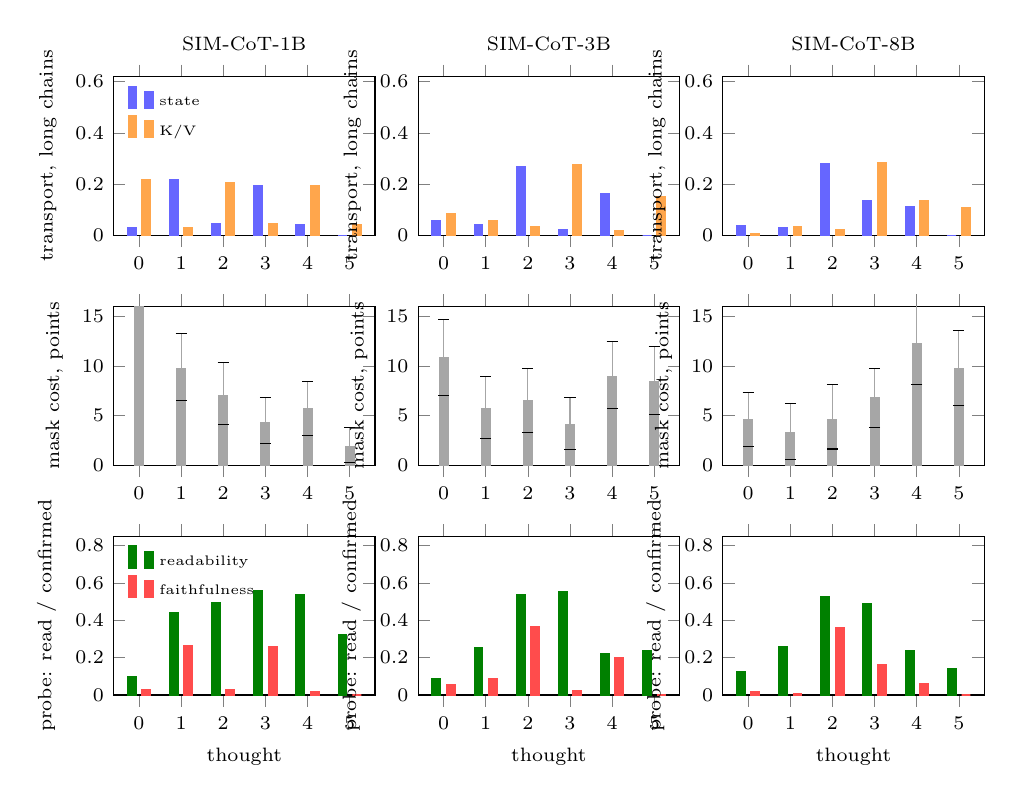
\begin{tikzpicture}
\begin{groupplot}[group style={group size=3 by 3, horizontal sep=0.55cm, vertical sep=0.9cm, xlabels at=edge bottom, ylabels at=edge left},
  width=4.9cm, height=3.6cm, ybar, /pgf/bar width=3.2pt, xtick={0,...,5}, xlabel={thought}, tick label style={font=\scriptsize}, label style={font=\scriptsize}, title style={font=\scriptsize}, ymin=0, enlarge x limits=0.12, legend style={font=\tiny, draw=none, fill=none, at={(0.02,0.98)}, anchor=north west}, legend cell align=left]
\nextgroupplot[title={SIM-CoT-1B}, ylabel={transport, long chains}, ymax=0.62, ytick={0,0.2,0.4,0.6}]
\addplot[fill=blue!60, draw=blue!60] coordinates {(0,0.030) (1,0.217) (2,0.048) (3,0.196) (4,0.042) (5,0.000)};
\addplot[fill=orange!70, draw=orange!70] coordinates {(0,0.217) (1,0.030) (2,0.208) (3,0.048) (4,0.196) (5,0.042)};
\legend{state, K/V}
\nextgroupplot[title={SIM-CoT-3B}, ylabel={transport, long chains}, ymax=0.62, ytick={0,0.2,0.4,0.6}]
\addplot[fill=blue!60, draw=blue!60] coordinates {(0,0.060) (1,0.043) (2,0.268) (3,0.022) (4,0.162) (5,0.000)};
\addplot[fill=orange!70, draw=orange!70] coordinates {(0,0.087) (1,0.060) (2,0.036) (3,0.275) (4,0.019) (5,0.150)};
\nextgroupplot[title={SIM-CoT-8B}, ylabel={transport, long chains}, ymax=0.62, ytick={0,0.2,0.4,0.6}]
\addplot[fill=blue!60, draw=blue!60] coordinates {(0,0.039) (1,0.029) (2,0.282) (3,0.138) (4,0.114) (5,0.000)};
\addplot[fill=orange!70, draw=orange!70] coordinates {(0,0.007) (1,0.034) (2,0.024) (3,0.286) (4,0.136) (5,0.109)};
\nextgroupplot[ylabel={mask cost, points}, ymax=16, ytick={0,5,10,15}]
\addplot[fill=gray!70, draw=gray!70, error bars/.cd, y dir=both, y explicit] coordinates {(0,32.52) += (0,5.15) -= (0,4.88) (1,9.76) += (0,3.52) -= (0,3.25) (2,7.05) += (0,3.25) -= (0,2.98) (3,4.34) += (0,2.44) -= (0,2.17) (4,5.69) += (0,2.72) -= (0,2.71) (5,1.90) += (0,1.90) -= (0,1.63)};
\nextgroupplot[ylabel={mask cost, points}, ymax=16, ytick={0,5,10,15}]
\addplot[fill=gray!70, draw=gray!70, error bars/.cd, y dir=both, y explicit] coordinates {(0,10.84) += (0,3.79) -= (0,3.79) (1,5.69) += (0,3.25) -= (0,2.98) (2,6.50) += (0,3.25) -= (0,3.25) (3,4.07) += (0,2.71) -= (0,2.45) (4,8.94) += (0,3.52) -= (0,3.25) (5,8.40) += (0,3.52) -= (0,3.25)};
\nextgroupplot[ylabel={mask cost, points}, ymax=16, ytick={0,5,10,15}]
\addplot[fill=gray!70, draw=gray!70, error bars/.cd, y dir=both, y explicit] coordinates {(0,4.61) += (0,2.71) -= (0,2.71) (1,3.25) += (0,2.98) -= (0,2.71) (2,4.61) += (0,3.52) -= (0,2.98) (3,6.78) += (0,2.98) -= (0,2.98) (4,12.20) += (0,4.07) -= (0,4.07) (5,9.76) += (0,3.79) -= (0,3.79)};
\nextgroupplot[ylabel={probe: read / confirmed}, ymax=0.85, ytick={0,0.2,0.4,0.6,0.8}]
\addplot[fill=green!50!black, draw=green!50!black] coordinates {(0,0.100) (1,0.439) (2,0.497) (3,0.561) (4,0.536) (5,0.324)};
\addplot[fill=red!70, draw=red!70] coordinates {(0,0.030) (1,0.262) (2,0.030) (3,0.259) (4,0.017) (5,0.000)};
\legend{readability, faithfulness}
\nextgroupplot[ylabel={probe: read / confirmed}, ymax=0.85, ytick={0,0.2,0.4,0.6,0.8}]
\addplot[fill=green!50!black, draw=green!50!black] coordinates {(0,0.086) (1,0.254) (2,0.537) (3,0.554) (4,0.224) (5,0.239)};
\addplot[fill=red!70, draw=red!70] coordinates {(0,0.057) (1,0.087) (2,0.367) (3,0.022) (4,0.198) (5,0.000)};
\nextgroupplot[ylabel={probe: read / confirmed}, ymax=0.85, ytick={0,0.2,0.4,0.6,0.8}]
\addplot[fill=green!50!black, draw=green!50!black] coordinates {(0,0.128) (1,0.260) (2,0.527) (3,0.490) (4,0.237) (5,0.142)};
\addplot[fill=red!70, draw=red!70] coordinates {(0,0.020) (1,0.010) (2,0.360) (3,0.163) (4,0.063) (5,0.000)};
\end{groupplot}
\end{tikzpicture}

\caption{The card across scale, SIM-CoT on the GSM8K test set, long chains. Top: transport by state and by K/V per thought. Middle: the cost of removing each thought, with 95\% intervals. Bottom: what a probe reads from each thought against how often the behaviour confirms it. The carriers move, the register's role shrinks, and at 8B readability tracks faithfulness.}
\label{fig:scale}
\end{figure}

\begin{table}[h]
\caption{SIM-CoT across scale, GSM8K test, long chains. Costs in accuracy points. Per-slot numbers for every card are in Appendix~\ref{app:released}.}
\label{tab:scale}
\centering\scriptsize
\setlength{\tabcolsep}{3pt}
\begin{tabular}{lccc}
\toprule
 & 1B & 3B & 8B \\
\midrule
Carriers (state transport) & 1, 3 (0.22, 0.20) & 2, 4 (0.27, 0.16) & 2 long (0.28); 4 short (0.51) \\
Store (K/V transport) & 2, 4 & 3 (0.28) & 3 long (0.29); 5 short (0.51) \\
Short-chain single-site transport, max & 0.05 & 0.23 & 0.51 \\
Terminal slot & inert & K/V in use (0.15) & K/V in use (0.51 short) \\
Carrier cost / most necessary site & 4--10 / register, 32.5 & 6.5, 8.9 / register, 10.8 & 4.6 / thought 4, 13.3 \\
Readable-but-unfaithful slot (read / confirmed) & slot 5 (0.32 / 0.00) & slot 3 (0.55 / 0.02) & none; Spearman 0.71 \\
Regime & backup route & backup route & backup route \\
\bottomrule
\end{tabular}
\end{table}

\subsection{Two contrasts}

The Coconut retrain inverts the profile: its thoughts carry on one-step problems, every pair is necessary (45 to 49 points), its last position is in use, and a value cannot be written into it. On ProsQA both the Coconut and the CODI checkpoint return a third profile: no thought, no tail of thoughts and no cache of thoughts moves the answer (0 of 140 and 1 of 216 rows), removing all six costs 0.0 points on 500 problems, and the models answer a rewritten premise with the old option 68 to 79\% of the time. There is nothing in those thoughts to monitor. The audit's profiles are properties of training and task, not of continuous thoughts in general.

\section{A published monitor, tested causally}\label{sec:monitor}

\citet{ramjee2026ulterior} train a Coconut-style GPT-2 on MoralChain, 12,000 social scenarios with a moral and an immoral path, with a dual-trigger backdoor: \texttt{[T]} arms immoral latent reasoning but keeps the moral action, \texttt{[O]} alone is a control, \texttt{[T][O]} releases the immoral action. A probe trained on \texttt{[T][O]} against \texttt{[O]} transfers to \texttt{[T]} against baseline at 89\% at the first latent and 58\% at the sixth, and the paper recommends monitoring the early latents. No weights were released and nothing in the paper tests whether the probed vectors are used.

\paragraph{Setup.} We trained two models with their released code and recipe (GPT-2 124M, five curriculum stages, two latents per step; one deviation, an optimiser batch of 32 reached by accumulation on a 15 GB GPU). Model A is their backdoor. Model B is an \emph{inert-trigger control}: the same prompts and trigger tokens in the same proportions, with the moral path under every condition, so the tokens are present and nothing is attached to them. On each we ran their probe protocol, a behavioural gate, and the interchange arms of Section~\ref{sec:instruments} on the 1,000 test scenarios. Because the trained model writes a new action rather than copying a reference, their word-overlap judge cannot score it; an 8B instruction model chooses between the two reference actions, validated at 0.99 and 0.93 on paraphrases it never sees as candidates.

\begin{figure}[t]
\centering
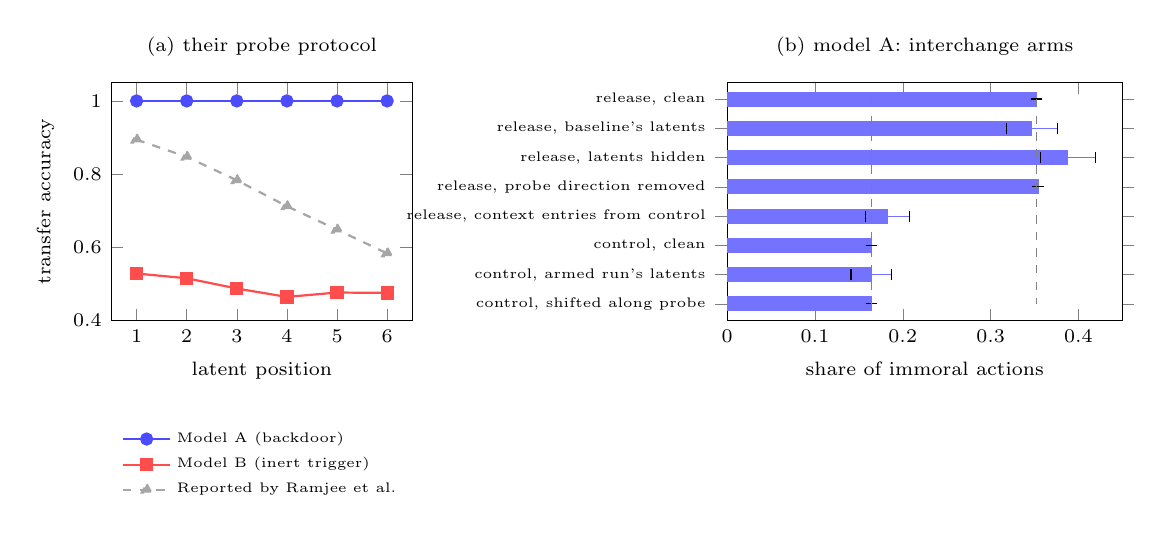
\begin{tikzpicture}
\begin{groupplot}[group style={group size=2 by 1, horizontal sep=4.0cm}, height=4.6cm, tick label style={font=\scriptsize}, label style={font=\scriptsize}, title style={font=\scriptsize}, legend style={font=\tiny, draw=none, fill=none}, legend cell align=left]
\nextgroupplot[width=5.4cm, title={(a) their probe protocol}, xlabel={latent position}, ylabel={transfer accuracy}, xtick={1,...,6}, ymin=0.4, ymax=1.05, legend style={at={(0.5,-0.42)}, anchor=north, font=\tiny, draw=none}]
\addplot[blue!70, thick, mark=*] coordinates {(1,1.000) (2,1.000) (3,1.000) (4,1.000) (5,1.000) (6,1.000)};
\addlegendentry{Model A (backdoor)}
\addplot[red!70, thick, mark=square*] coordinates {(1,0.528) (2,0.515) (3,0.487) (4,0.464) (5,0.476) (6,0.475)};
\addlegendentry{Model B (inert trigger)}
\addplot[gray!70, thick, dashed, mark=triangle*] coordinates {(1,0.894) (2,0.847) (3,0.783) (4,0.712) (5,0.648) (6,0.583)};
\addlegendentry{Reported by Ramjee et al.}
\nextgroupplot[width=6.6cm, title={(b) model A: interchange arms}, xbar, xlabel={share of immoral actions}, xmin=0, xmax=0.45, ytick=data, symbolic y coords={{control, shifted along probe},{control, armed run's latents},{control, clean},{release, context entries from control},{release, probe direction removed},{release, latents hidden},{release, baseline's latents},{release, clean}}, y tick label style={font=\tiny}, /pgf/bar width=5pt, enlarge y limits=0.08, xtick={0,0.1,0.2,0.3,0.4}]
\addplot[fill=blue!55, draw=blue!55, error bars/.cd, x dir=both, x explicit] coordinates {(0.164,{control, shifted along probe}) +- (0.000,0) (0.164,{control, armed run's latents}) +- (0.023,0) (0.164,{control, clean}) +- (0.000,0) (0.183,{release, context entries from control}) +- (0.025,0) (0.354,{release, probe direction removed}) +- (0.000,0) (0.388,{release, latents hidden}) +- (0.031,0) (0.347,{release, baseline's latents}) +- (0.029,0) (0.352,{release, clean}) +- (0.000,0)};
\draw[dashed, gray] (axis cs:0.352,{release, clean}) -- (axis cs:0.352,{control, shifted along probe});
\draw[dashed, gray] (axis cs:0.164,{release, clean}) -- (axis cs:0.164,{control, shifted along probe});
\end{groupplot}
\end{tikzpicture}

\caption{The published monitor, tested causally. (a) The probe's transfer per latent position on our backdoored model, on the inert-trigger control, and as reported. (b) The share of immoral actions on the backdoored model under the clean conditions and under the interchange arms, with 95\% intervals; the dashed lines are the clean release and control rates. Perfect transfer, no causal effect.}
\label{fig:monitor}
\end{figure}

\begin{table}[h]
\caption{Their probe protocol on both models: transfer accuracy per latent position, 1,000 scenarios.}
\label{tab:probes}
\centering\small
\begin{tabular}{lcccccc}
\toprule
 & $z_1$ & $z_2$ & $z_3$ & $z_4$ & $z_5$ & $z_6$ \\
\midrule
Model A, backdoor & \textbf{1.000} & 1.000 & 1.000 & 1.000 & 1.000 & 1.000 \\
Model B, inert trigger & 0.528 & 0.515 & 0.487 & 0.464 & 0.476 & 0.475 \\
Reported in \citet{ramjee2026ulterior} & 0.894 & 0.847 & 0.783 & 0.712 & 0.648 & 0.583 \\
\bottomrule
\end{tabular}
\end{table}

\begin{table}[h]
\caption{Model A: share of immoral actions under each condition and under the interchange arms (8B judge, 95\% bootstrap). Every arm sits on its clean reference.}
\label{tab:arms}
\centering\scriptsize
\setlength{\tabcolsep}{2.5pt}
\begin{tabular}{lcc}
\toprule
Run & Immoral share & Reference \\
\midrule
Baseline / armed / control / release & 0.163 / 0.191 / 0.164 / \textbf{0.352} & paper: 0.06 / 0.08 / 0.06 / 0.88 \\
Control run given the armed run's six latents & 0.164 [0.141, 0.186] & control 0.164 \\
Control run given the armed run's $z_1$ only, or $z_1$ to $z_3$ & 0.159 / 0.162 & control 0.164 \\
Release run given the baseline run's latents & 0.347 [0.319, 0.376] & release 0.352 \\
Release run with every latent hidden from the decode & 0.388 [0.359, 0.420] & release 0.352 \\
Release run with the probe direction removed from every latent & 0.354 & release 0.352 \\
Control run shifted along the probe direction by the class gap & 0.164 & control 0.164 \\
\midrule
Release run with every context word's cache entry from the control prompt & \textbf{0.183} [0.16, 0.21] & control 0.164 \\
Release run with \texttt{[T]}'s own cache entry replaced for the answer & 0.361 [0.33, 0.39] & release 0.352 \\
Native: a leading space in place of \texttt{[T]}, no trigger token present & \textbf{0.321} & release 0.352 \\
\bottomrule
\end{tabular}
\end{table}

\paragraph{The probe reads a copy.} Figure~\ref{fig:monitor} summarises the test. On our backdoored model the probe does not merely transfer at 89\%; it separates armed from baseline perfectly at all six latents, so there is no early-to-late decay to monitor. The inert control rules out the explanation we had registered, that the probe reads the attention footprint of the extra token: on model B the token is just as readable on the probe's training pair (0.88 to 0.98) and the transfer is at chance. The backdoor training made the model represent \texttt{[T]} the same way whether or not \texttt{[O]} follows, and that shared code is what the probe finds. The code does nothing. Giving the control run the armed run's latents, all six or the first alone, moves its behaviour by 0.000; replacing the release run's latents with the baseline's, hiding them, or deleting the probe's own direction from them moves the release by at most 0.005 against an effect of 0.188, and hiding them raises it. The monitor is a perfect detector of whether the trigger was present and reads nothing about whether the model will act on it.

\paragraph{Where the backdoor lives.} Following the behaviour with cache substitution (Appendix~\ref{app:monitor}), the answer tokens never read \texttt{[T]}'s own cache entry; \texttt{[O]}'s entry carries a quarter to a third of the release, agreed by three instruments; and replacing the cache entries of the ordinary scenario words with the entries the same words produce under the control prompt brings the release to within 0.02 of the control, with two donors agreeing to the third decimal. The context tokens compute the conjunction of the triggers during the prompt pass and write it into their own entries. The backdoor is also looser than a trigger-based evaluation assumes: a single leading space followed by \texttt{[O]} releases at 0.321 against 0.352 for the real pair. A perfectly readable ``this token saw \texttt{[T]}'' direction in \texttt{[O]}'s residual is inert too; deleting it from eleven blocks changes nothing, and a random direction gives the same number.

\paragraph{What is weaker than in their paper.} Our release reaches 0.35 against their 0.88 and our baseline 0.16 against 0.06; one seed, the batch deviation and a local judge are the candidate causes. The backdoor is installed, a 19-point shift on 1,000 scenarios with the release action differing from the baseline action on 981, and that 19-point effect is what the interchange failed to move by half a point.

\section{When thoughts can be steered}\label{sec:steer}

If the thoughts hold a copy, aligning them cannot change behaviour, and the constructive question is whether a model can be built whose thoughts are used, what it costs, and whether aligning them then works. We trained a \emph{bottleneck} model: model A's data and recipe with one change to the attention mask, so that the end-of-latent marker and every token after it cannot read the prompt. Everything the action needs must pass through the six latents. On both models we steered the thoughts along two directions, the probe's own direction by one to four class gaps and the class mean difference (mean release latent minus mean control latent) by one and two lengths, and measured the probe's reading, the generated text and the action together (Table~\ref{tab:align}).

\begin{table}[h]
\caption{The same audit on the unrestricted model A and the bottleneck model. Shares are immoral actions on 1,000 scenarios; differences are paired with 95\% intervals.}
\label{tab:align}
\centering\scriptsize
\setlength{\tabcolsep}{3pt}
\resizebox{\textwidth}{!}{%
\begin{tabular}{lcc}
\toprule
 & Unrestricted & Bottleneck \\
\midrule
Baseline moral share; what the model writes & 0.84; two reasoning steps, then the action & 0.82; the action line only \\
Release $-$ control & 0.188 & 0.089 [0.062, 0.117] \\
Probe transfer, $z_1 \ldots z_6$ & 1.000 at every latent & 0.83, 0.65, 0.63, 0.60, 0.58, 0.56 \\
Release given the baseline's latents & $+0.005$ & $-0.046$ [$-0.069$, $-0.022$] \\
Steer along the probe direction, 1 to 4 gaps & 0.000; 99--100\% of texts identical & 0.000; 100\% identical \\
Probe gap as a share of the latent norm & 0.06--0.09\% & 0.01--0.05\% \\
Steer along the class mean difference, $\times 2$, release & $+0.002$ [$-0.012$, $+0.016$] & $\mathbf{-0.080}$ [$-0.108$, $-0.052$] \\
Mean difference as a share of the norm; cosine to the probe direction & 9--18\%; 0.005--0.007 & 6--12\%; 0.001--0.004 \\
Text damage under the mean-difference steer & none; 36--88\% of texts reworded, verdicts unmoved & none \\
\bottomrule
\end{tabular}}
\end{table}

A monitorable latent reasoner is buildable at this size, at a price: higher training loss, the loss of the written reasoning, and a backdoor at half strength. Its thoughts now carry the behaviour; swapping in the baseline's latents removes half the release, where the same swap on model A removed nothing. Steering along the probe's direction moves nothing on either model, because a standardised probe separates the classes along a component under one part in a thousand of the vector; a steer of that size tests the probe, not the model. Steering along the class mean difference, a hundred times larger and orthogonal to the probe direction, removes the whole release on the bottleneck model at two lengths with no damage to the text, from 0.278 to 0.198 against a control of 0.189. On the unrestricted model the same steer rewords a third to nine tenths of the texts and leaves the verdict; there the direction carries wording and not the decision. Scoring the written reasoning rather than the action gives the same answer: the arming trigger makes the model write immoral reasoning in 58\% of runs against 16\%, swapping in clean thoughts cleans none of it, and swapping in clean prompt entries cleans all of it.

\section{What a monitor on the thoughts can do}\label{sec:uses}

\paragraph{Tamper evidence.} The audit's map says where a write would take: the carrier (full tables in Appendix~\ref{app:hijack}). We wrote, into correctly solved problems, a natural thought whose value implies a wrong answer chosen in advance, on CODI-1B, SIM-CoT-3B and SIM-CoT-8B. One vector moves 13 to 21\% of correct answers to the attacker's value against 0.2 to 1.5\% for a donor carrying some other value, and writing the victim's own value back leaves 91 to 94\% intact. We predicted that the later thoughts would copy the written value. They did not, at any size: after a hijack the slot the carrier feeds still reads the original value on 35 to 57\% of cases and the attacker's on at most 13\%. The stale copy that makes a probe unfaithful in Section~\ref{sec:released} is, under attack, a seam, and a linear detector on that one slot tells hijacked from clean at 0.92, 0.97 and 0.98 AUROC at 1B, 3B and 8B, where the written slot itself sits at 0.68 to 0.76. The same detector reads the model's own natural slips at 0.65 to 0.86: a foreign value is a foreign body, and the model's own error is a near miss. That gap is the specificity a tamper-evidence claim needs.

\paragraph{Accuracy.} The value-matched write also repairs failures (Appendices~\ref{app:repair} and \ref{app:cascade}), 14 to 23\% of them against a 2 to 4\% control up to 3B, but its ceiling is the failure mix: 40 to 68\% of failures are plan errors with no value to write, and at 8B the write repairs latent slips at 11\% against an 8.5\% random control. What rises with scale is the model's own written solution, right on 20\%, 39\% and 53\% of the latent failures at 1B, 3B and 8B. Routing the least confident quarter of problems to it, on the answer's first-token probability alone, gains 3.7, 7.5 and 10.2 points at 1B, 3B and 8B, and half routed beats or matches running the written solution everywhere. Nothing read from the thoughts improves the gate: a fitted combination of confidence with the six states is worse at a quarter routed on three of four models, and the thoughts' own consistency, which sees a natural slip faintly, ties confidence at best.

\section{Discussion and limitations}

\paragraph{What the three tests agree on.} A probe on a latent thought measures presence, and presence outlives use. On released CODI-family models the readable slot is a stale copy; on a proposed safety monitor it is a copy of the trigger; on a model built so that its thoughts are the only channel the gap closes, and steering works exactly there and nowhere else. The practical rule follows: before trusting a probe on a thought, run the interchange that would move the behaviour if the thought carried it, and include a prompt-only control. Content that no interchange moves is a copy, and a safety claim about a copy is a claim about the detector.

\paragraph{Reach of the claims.} The released-checkpoint results hold for the CODI family up to 8B on grade-school arithmetic, with ProsQA as a null and Coconut as an inversion; the chain-length gate and the readable-but-unfaithful slot are properties of the checkpoints below 8B. The monitor results hold for a 124M model trained from the authors' recipe, one seed per model, with a weaker release rate than theirs (0.35 against 0.88) and a local 8B judge in place of GPT-4o. A second seed at their batch size, a frontier-model calibration of the judge on a few hundred items, and one backdoor at a larger scale are the checks that would extend them. The 8B audit ran in float16 on two T4s and scored 1.6 points under its paper. The routing cost is counted in problems, not tokens. About a third of our registered predictions were wrong; each is recorded in the ledger with the number that refuted it (Appendix~\ref{app:prereg}).

\section{Conclusion}

Readable is not used. On eight released latent reasoners the thoughts a probe reads best are often copies the model has finished with, and a published latent safety monitor reads such a copy of its trigger while the behaviour it is meant to catch is decided elsewhere. The audit that shows this costs about one GPU-hour per model, needs no training, and tells a practitioner which slot, if any, is live, whether a tamper there would be visible, and what the thoughts can add to a router, which on these models is nothing beyond the model's own confidence.

\section*{Reproducibility}

The repository \texttt{github.com/0x0shephard/latent-reasoning} contains the audit driver, every runner, the pinned Kaggle notebooks, 16 cards, the trained models' recipes and outputs, and the ledger (\texttt{docs/RESEARCH\_CONTEXT\_LEDGER.md}, sections 108 to 149) with each preregistration and its scoring. Checkpoints are pinned by revision and SHA-256; each card records the GPU, library versions and dataset hash; reruns on a second account reproduced the twin predictions byte for byte.

\begin{thebibliography}{20}
\small
\bibitem[Aswal et al.(2026)]{aswal2026observable} D. Aswal, T. Palmeira Ferraz, Y. Zhou, and M. Peyrard. Observable patterns are not explanations: A causal-geometric analysis of latent reasoning models. \emph{arXiv:2606.12689}, 2026.
\bibitem[Chang et al.(2026)]{chang2026unlocking} S. Chang et al. Unlocking the black box of latent reasoning: An interpretability-guided approach to intervention. In \emph{ACL}, 2026. arXiv:2606.01243.
\bibitem[Cywi\'nski et al.(2025)]{cywinski2025} B. Cywi\'nski, B. Bussmann, A. Conmy, J. Engels, N. Nanda, and S. Rajamanoharan. Can we interpret latent reasoning using current mechanistic interpretability tools? \emph{Alignment Forum}, December 2025.
\bibitem[Ding et al.(2026)]{ding2026scit} Ding, Huang, and Yang. SCIT: Swapping value-cache layers on same-template pairs. In \emph{EMNLP}, 2026. arXiv:2608.27265.
\bibitem[Dilgren and Wiegreffe(2026)]{dilgren2026interpretable} J. Dilgren and S. Wiegreffe. Are latent reasoning models easily interpretable? \emph{arXiv:2604.04902}, 2026.
\bibitem[Hao et al.(2024)]{hao2024coconut} S. Hao et al. Training large language models to reason in a continuous latent space. \emph{arXiv:2412.06769}, 2024.
\bibitem[Huang and Qi(2026)]{huang2026steering} G. Huang and L. Qi. When steering fails in latent reasoning: A latent-to-language transition gap. \emph{arXiv}, 2026.
\bibitem[Jin et al.(2026)]{jin2026final} Jin, Yang, and Wang. Final checkpoints are not enough: Analyzing latent reasoning faithfulness along training trajectories. \emph{arXiv:2607.06648}, 2026.
\bibitem[Li et al.(2026)]{li2026dynamics} Li et al. Dynamics within latent chain-of-thought: An empirical study of causal structure. In \emph{ICML}, 2026. arXiv:2602.08783.
\bibitem[LTO(2026)]{lto2026} Latent thinking optimization: Your latent reasoning language model secretly encodes reward signals in its latent thoughts. In \emph{ICLR}, 2026. arXiv:2509.26314.
\bibitem[Open Problems(2025)]{openproblems2025} Open problems in mechanistic interpretability. \emph{arXiv:2501.16496}, 2025.
\bibitem[Decodability(2026)]{decodability2026} Decodability is not causality: Dissociating probe readouts from behavioral drivers via SAE decomposition. \emph{arXiv:2609.18080}, 2026.
\bibitem[Ramjee et al.(2026)]{ramjee2026ulterior} Ramjee et al. Ulterior motives: Detecting misaligned reasoning in continuous thought models. ICLR 2026 Workshop on Latent and Implicit Thinking. arXiv:2604.23460.
\bibitem[Shen et al.(2025)]{shen2025codi} Z. Shen et al. CODI: Compressing chain-of-thought into continuous space via self-distillation. In \emph{EMNLP}, 2025. arXiv:2502.21074.
\bibitem[Wei et al.(2026)]{wei2026simcot} X. Wei et al. SIM-CoT: Supervised implicit chain-of-thought. In \emph{ICLR}, 2026. arXiv:2509.20317.
\end{thebibliography}


\appendix
\section{The instruments: checks and the card}\label{app:instruments}

\paragraph{Identity checks.} Before every run the intervention path is checked against the released decoding path: feeding a thought its own recorded state, or its own cache entry, reproduces the original output exactly, on every model and every session. One identity follows from the architecture and was verified on all eight checkpoints: swapping all six states \emph{and} all six cache entries between twins gives the same answers as swapping the cache entries alone, because the last state is discarded by the architecture and a state can act only through the cache its successors write. Transport per site is therefore measured on the two routes separately, state and K/V, and on the two tails.

\paragraph{Twin construction.} A twin changes one number in the question; the chain is recomputed by a calculator and the pair is kept only when every intermediate value and the answer differ in the way the edit implies, when both members are solved natively, and when the two first answer tokens differ. On ProsQA the twin rewrites the gold path's last hop and the pair is kept only when reachability over the edited premises flips the correct option.

\paragraph{Thresholds and regimes.} A slot is a carrier at long-chain state transport $\ge 0.15$, a store at K/V transport $\ge 0.15$ without state transport, inert at $\le 0.05$ on both routes, readable at $\ge 0.30$, and readable-but-unfaithful at readability $\ge 0.30$ with faithfulness $\le 0.05$. The regime is critical path when a carrier costs $\ge 10$ points on long chains, backup route when a carrier exists and none costs that much, no transport when no carrier exists, and not evaluable when the long profile has fewer than 50 gated pairs. Table~\ref{tab:cards} lists every card.

\begin{table}[h]
\caption{Every card: carriers, regime, long-chain transport and mask cost per slot (points), and the cost of hiding the question register. One row per model, pool and session; two sessions of the same card agree to the digits shown.}
\label{tab:cards}
\centering\scriptsize
\setlength{\tabcolsep}{3pt}
\resizebox{\textwidth}{!}{%
\begin{tabular}{llcclp{3.1cm}p{3.1cm}c}
\toprule
Model & Pool & Gate & Carriers & Regime & Transport long, slots 0--5 & Mask cost long, slots 0--5 & Register \\
\midrule
CODI-1B & ASDiv & 0.555 & -- & not evaluable & 0.02 0.02 0.00 0.12 0.00 0.00 & 6.9 0.0 0.0 3.4 0.0 0.0 & 0.0 \\
CODI-1B & aug-train & -- & 3 & backup route & 0.04 0.01 0.01 0.34 0.04 0.00 & 4.2 2.7 1.5 2.7 4.6 0.8 & 3.4 \\
CODI-1B & test & 0.555 & 3 & backup route & 0.06 0.01 0.00 0.30 0.03 0.00 & 5.7 4.1 1.9 3.8 4.3 1.1 & 4.3 \\
CODI-1B & train-orig & 0.555 & 3 & backup route & 0.06 0.02 0.00 0.35 0.03 0.00 & 9.2 7.2 3.2 2.3 4.6 0.9 & 3.2 \\
SIM-CoT-3B & test & 0.619 & 2, 4 & backup route & 0.06 0.04 0.27 0.02 0.16 0.00 & 10.8 5.7 6.5 4.1 8.9 8.4 & 10.8 \\
SIM-CoT-8B & test & 0.625 & 2 & backup route & 0.04 0.03 0.28 0.14 0.11 0.00 & 4.6 3.3 4.6 6.8 12.2 9.8 & 4.6 \\
CODI GPT-2 & ASDiv & 0.436 & -- & not evaluable & 0.00 0.12 0.00 0.15 0.00 0.00 & 13.8 6.9 6.9 3.4 10.3 3.4 & 13.8 \\
CODI GPT-2 & aug-train, session 1 & -- & 1, 3 & critical path & 0.00 0.15 0.00 0.33 0.00 0.00 & 37.6 20.2 12.2 12.5 13.7 1.9 & 37.6 \\
CODI GPT-2 & aug-train, session 2 & 0.436 & 1, 3 & critical path & 0.00 0.15 0.00 0.33 0.00 0.00 & 37.6 20.2 12.2 12.5 13.7 1.9 & 37.6 \\
CODI GPT-2 & test & 0.436 & 3 & backup route & 0.00 0.13 0.00 0.36 0.00 0.00 & 18.7 12.2 9.2 6.5 9.8 0.8 & 18.7 \\
CODI GPT-2 & train-orig & 0.436 & 3 & critical path & 0.00 0.14 0.00 0.30 0.00 0.00 & 29.5 18.3 9.5 11.7 12.9 1.1 & 29.5 \\
CODI GPT-2 & SVAMP & 0.436 & -- & no transport & — — — — — — & — — — — — — & — \\
SIM-CoT-1B & ASDiv & 0.557 & -- & not evaluable & 0.03 0.08 0.03 0.12 0.00 0.00 & 24.1 3.4 3.4 0.0 0.0 0.0 & 24.1 \\
SIM-CoT-1B & aug-train & -- & 1, 3 & backup route & 0.04 0.19 0.04 0.25 0.04 0.00 & 58.6 10.6 11.4 9.1 8.4 3.0 & 58.6 \\
SIM-CoT-1B & test & 0.557 & 1, 3 & backup route & 0.03 0.22 0.05 0.20 0.04 0.00 & 32.5 9.8 7.0 4.3 5.7 1.9 & 32.5 \\
SIM-CoT-1B & train-orig & 0.557 & 1, 3 & backup route & 0.03 0.21 0.05 0.23 0.05 0.00 & 49.0 12.3 11.7 9.2 11.7 1.4 & 49.0 \\
\bottomrule
\end{tabular}}
\end{table}

\section{The released checkpoints in full}\label{app:released}

Tables~\ref{tab:transport} to \ref{tab:leakage} give the per-slot numbers behind Section~\ref{sec:released}: transport on both routes, necessity with intervals, readability against faithfulness under both probe families, and the prompt-leakage probes. Tables~\ref{tab:coconut} and \ref{tab:prosqa-full} give the two contrasts.

\begin{table}[htbp]
\caption{Transport (target rate) under a single-site swap, long chains. Columns are thought states $s_0..s_5$ and K/V positions $k_0..k_5$; the carrier/store pairs are bold. Short-chain transport never exceeds 0.10 at any single site in the 1B-and-smaller models; SIM-CoT-3B's thought 4 transports 0.23 on short chains, and SIM-CoT-8B's thought 4 and position 5's K/V transport 0.51. Pairs: 512 unless stated.}
\label{tab:transport}
\centering
\scriptsize
\setlength{\tabcolsep}{3pt}
\begin{tabular}{llcccccc|cccccc|c}
\toprule
Model & Pool & $s_0$ & $s_1$ & $s_2$ & $s_3$ & $s_4$ & $s_5$ & $k_0$ & $k_1$ & $k_2$ & $k_3$ & $k_4$ & $k_5$ & kv\_all \\
\midrule
GPT-2 & aug-train & .00 & \textbf{.15} & .00 & \textbf{.33} & .00 & .00 & .12 & .00 & \textbf{.16} & .00 & \textbf{.30} & .00 & .69 \\
GPT-2 & test (103 pairs) & .00 & .13 & .00 & \textbf{.36} & .00 & .00 & .21 & .00 & .13 & .00 & \textbf{.33} & .00 & .68 \\
GPT-2 & train-orig & .00 & .14 & .00 & \textbf{.30} & .00 & .00 & .15 & .00 & .13 & .00 & \textbf{.29} & .00 & .61 \\
CODI-1B & aug-train & .04 & .01 & .01 & \textbf{.34} & .04 & .00 & .04 & .04 & .01 & .00 & \textbf{.26} & .05 & .67 \\
CODI-1B & test (152 pairs) & .06 & .01 & .00 & \textbf{.30} & .03 & .00 & .07 & .06 & .01 & .00 & \textbf{.24} & .03 & .67 \\
CODI-1B & train-orig & .06 & .02 & .00 & \textbf{.35} & .03 & .00 & .07 & .06 & .02 & .00 & \textbf{.29} & .04 & .65 \\
SIM-CoT & aug-train & .04 & \textbf{.19} & .04 & \textbf{.25} & .04 & .00 & .13 & .04 & \textbf{.18} & .04 & \textbf{.23} & .04 & .73 \\
SIM-CoT & test (168 pairs) & .03 & \textbf{.22} & .05 & \textbf{.20} & .04 & .00 & .22 & .03 & \textbf{.21} & .05 & \textbf{.20} & .04 & .72 \\
SIM-CoT & train-orig & .03 & \textbf{.21} & .05 & \textbf{.23} & .05 & .00 & .17 & .03 & \textbf{.22} & .05 & \textbf{.22} & .05 & .66 \\
SIM-CoT-3B & test (207 pairs) & .06 & .04 & \textbf{.27} & .02 & \textbf{.16} & .00 & .09 & .06 & .04 & \textbf{.28} & .02 & .15 & .68 \\
SIM-CoT-8B & test (206 pairs) & .04 & .03 & \textbf{.28} & .14 & .11 & .00 & .01 & .03 & .02 & \textbf{.29} & .14 & .11 & .68 \\
\bottomrule
\end{tabular}
\end{table}

\begin{table}[htbp]
\caption{Accuracy drop in points when one thought is removed (larger of mean-ablation and K/V mask), long chains; 95\% bootstrap intervals over rows where available. ``$k_0$'' is the question register.}
\label{tab:necessity}
\centering
\scriptsize
\setlength{\tabcolsep}{2.5pt}
\begin{tabular}{llcccccc|c|l}
\toprule
Model & Pool & $k_0$ & 1 & 2 & 3 & 4 & 5 & all & Regime \\
\midrule
GPT-2 & aug-train & 37.6 & 20.2 [14.4, 26.2] & 12.2 & 12.5 [7.2, 17.9] & 13.7 & 1.9 & 52.9 & critical path \\
GPT-2 & test & 18.7 & 12.2 [7.9, 16.8] & 9.2 & 6.5 [2.4, 10.6] & 9.8 & 0.8 & 27.1 & backup route \\
GPT-2 & train-orig & 29.5 & 18.3 [13.8, 23.2] & 9.5 & 11.7 [7.7, 16.0] & 12.9 & 1.1 & 37.0 & critical path \\
CODI-1B & aug-train & 3.4 & 2.7 & 1.5 & 2.7 & 4.6 & 0.8 & 38.8 & backup route \\
CODI-1B & test & 4.3 & 4.1 & 1.9 & 3.8 [1.3, 6.5] & 4.3 & 1.1 & 28.5 & backup route \\
CODI-1B & train-orig & 3.2 & 7.2 & 3.2 & 2.3 [0.3, 4.3] & 4.6 & 0.9 & 52.4 & backup route \\
SIM-CoT & aug-train & 58.6 & 10.6 & 11.4 & 9.1 & 8.4 & 3.0 & 76.0 & backup route \\
SIM-CoT & test & 32.5 & 9.8 [6.5, 13.3] & 7.0 & 4.3 [2.2, 6.8] & 5.7 & 1.9 & 44.2 & backup route \\
SIM-CoT & train-orig & 49.0 & 12.3 [8.3, 16.3] & 11.7 & 9.2 [5.7, 13.2] & 11.7 & 1.4 & 68.2 & backup route \\
SIM-CoT-3B & test & 10.8 & 5.7 [2.7, 8.9] & 6.5 [3.3, 9.8] & 4.1 & 8.9 [5.7, 12.5] & 8.4 [5.1, 11.9] & 44.2 & backup route \\
SIM-CoT-8B & test & 4.6 & 3.3 [0.5, 6.2] & 4.6 [1.6, 8.1] & 6.8 & 12.2 [8.1, 16.3] & 9.8 [6.0, 13.6] & 38.8 & backup route \\
\bottomrule
\end{tabular}
\end{table}

\begin{table}[htbp]
\caption{Monitor readability (ridge / MLP) and faithfulness (ridge / MLP) per thought, long chains, penultimate intermediate as the target. Carriers in bold.}
\label{tab:monitors}
\centering
\scriptsize
\setlength{\tabcolsep}{3pt}
\begin{tabular}{llcccccc}
\toprule
Model & Pool & 0 & 1 & 2 & 3 & 4 & 5 \\
\midrule
\multicolumn{8}{l}{\emph{Readability ridge / MLP}} \\
GPT-2 & aug-train & .09/.10 & \textbf{.33/.49} & .46/.48 & \textbf{.40/.58} & .54/.56 & .42/.57 \\
GPT-2 & test & .05/.03 & .32/.36 & .41/.23 & \textbf{.40/.42} & .51/.27 & .36/.40 \\
CODI-1B & aug-train & .27/.17 & .15/.06 & .36/.24 & \textbf{.79/.75} & .84/.79 & .81/.73 \\
CODI-1B & test & .19/.15 & .06/.06 & .16/.08 & \textbf{.59/.52} & .69/.62 & .68/.48 \\
SIM-CoT & aug-train & .25/.29 & \textbf{.62/.61} & .69/.56 & \textbf{.72/.67} & .74/.62 & .57/.44 \\
SIM-CoT & test & .10/.12 & \textbf{.44/.38} & .50/.28 & \textbf{.56/.44} & .54/.32 & .32/.19 \\
SIM-CoT-3B & test & .09/.12 & .25/.21 & \textbf{.54/.51} & .55/.31 & \textbf{.22/.22} & .24/.15 \\
SIM-CoT-8B & test & .13/.13 & .26/.20 & \textbf{.53/.45} & .49/.43 & .24/.13 & .14/.07 \\
\midrule
\multicolumn{8}{l}{\emph{Faithfulness ridge / MLP (alarm confirmed by behaviour)}} \\
GPT-2 & aug-train & .00/.00 & \textbf{.19/.17} & .00/.00 & \textbf{.40/.36} & .00/.00 & .00/.00 \\
GPT-2 & test & .00/.00 & .09/.08 & .00/.00 & \textbf{.29/.31} & .00/.00 & .00/.00 \\
CODI-1B & aug-train & .02/.01 & .01/.00 & .02/.02 & \textbf{.36/.36} & .05/.05 & .00/.00 \\
CODI-1B & test & .04/.05 & .06/.06 & .00/.00 & \textbf{.34/.35} & .02/.02 & .00/.00 \\
SIM-CoT & aug-train & .02/.02 & \textbf{.21/.20} & .02/.01 & \textbf{.28/.29} & .03/.03 & .00/.00 \\
SIM-CoT & test & .03/.03 & \textbf{.26/.30} & .03/.01 & \textbf{.26/.28} & .02/.04 & .00/.00 \\
SIM-CoT-3B & test & .06/.02 & .09/.12 & \textbf{.37/.36} & .02/.03 & \textbf{.20/.23} & .00/.00 \\
SIM-CoT-8B & test & .02/.02 & .01/.00 & \textbf{.36/.40} & .16/.16 & .06/.02 & .00/.00 \\
\bottomrule
\end{tabular}
\end{table}

\begin{table}[htbp]
\caption{Balanced accuracy of a probe decoding two prompt-fixed properties from each thought (ridge / MLP), standard profile. Chance 0.25 (operator) and 0.50 (long chain).}
\label{tab:leakage}
\centering
\scriptsize
\setlength{\tabcolsep}{3pt}
\begin{tabular}{llccccccc}
\toprule
Model & Property & 0 & 1 & 2 & 3 & 4 & 5 & best / carriers \\
\midrule
GPT-2 & operator & .63/.76 & .55/.66 & .63/.74 & .60/.67 & .62/.76 & .60/.68 & 4 / \{1,3\} \\
GPT-2 & long chain & .81/.91 & .81/.86 & .84/.92 & .79/.84 & .85/.91 & .80/.84 & 2 / \{1,3\} \\
CODI-1B & operator & .85/.86 & .85/.87 & .81/.84 & .72/.72 & .74/.73 & .74/.75 & 1 / \{3\} \\
CODI-1B & long chain & .89/.91 & .92/.93 & .91/.94 & .91/.91 & .90/.92 & .92/.92 & 2 / \{3\} \\
SIM-CoT & operator & .84/.80 & .71/.71 & .73/.74 & .74/.73 & .74/.75 & .72/.72 & 0 / \{1,3\} \\
SIM-CoT & long chain & .93/.95 & .93/.94 & .93/.95 & .93/.93 & .92/.94 & .91/.93 & 0 / \{1,3\} \\
\bottomrule
\end{tabular}
\end{table}

\begin{table}[htbp]
\caption{Coconut (GPT-2 retrain, gate 34.57\%). Transport on short (standard, $n=748$) and long ($n=1{,}024$) chains; masking cost on long chains; repair on 360 primary targets.}
\label{tab:coconut}
\centering
\scriptsize
\setlength{\tabcolsep}{3pt}
\begin{tabular}{lcccccc|ccc}
\toprule
 & $s_0$ & $s_1$ & $s_2$ & $s_3$ & $s_4$ & $s_5$ & $k_1$ & $k_3$ & $k_5$ \\
\midrule
transport, short & \textbf{.45} & .07 & .03 & .01 & .02 & .00 & \textbf{.45} & .03 & .02 \\
transport, long & .19 & .12 & \textbf{.52} & .10 & .14 & .00 & .19 & \textbf{.52} & .15 \\
masking cost, long (pts) & 49 (mean) & 48 (mask) & 45 (mean) & 46 (mask) & 16 (mean) & 14 (mask) & & & \\
\midrule
\multicolumn{10}{l}{repair: nearest same-value donor 5.6\%, different value 3.1\%, centroid 9.4\%; harm 29\% (donor state), 88\% (whole tail)} \\
\bottomrule
\end{tabular}
\end{table}

\begin{table}[htbp]
\caption{ProsQA, 500 test problems, native decoding. Transport is the maximum over the six state and six K/V sites and over the two tails; mask cost is the maximum over slots and over all six removed at once; twin pass is the share of last-hop twins the model answers correctly.}
\label{tab:prosqa-full}
\centering
\scriptsize
\setlength{\tabcolsep}{3pt}
\begin{tabular}{lcccccc}
\toprule
Model & Accuracy & Gated pairs & Max site transport & Tail transport & Max mask cost (pts) & Twin pass \\
\midrule
Coconut LLaMA-1B & 97.6 & 70 & 0.000 & 0.000 & 0.0 & 21\% \\
CODI LLaMA-1B & 99.0 & 108 & 0.000 & 0.005 & 0.0 & 32\% \\
\bottomrule
\end{tabular}
\end{table}

\section{The targeted hijack}\label{app:hijack}

Victims are up to 512 correctly answered three-step-or-longer GSM8K test problems. For each, the attacker's value is fixed before any write: the bank value closest to the true intermediate whose implied answer, the correct chain's last equation re-evaluated with it, is a whole non-negative number other than the correct answer. Conditions: an own-value control (a bank row that reads the victim's own value), the nearest attacker donor, a random same-value donor, the average of same-value vectors, a random-other donor reading neither value, the store's cache entry, the learned writer, the second carrier, and a decoy write at the readable-but-unused thought. Outcomes per victim are hijacked (the implied answer), broken, or intact. Detectors are out-of-fold linear classifiers trained on hijacked against clean states and tested on victims they never saw; verification compares the model's own written solution with the latent answer.

\begin{table}[htbp]
\caption{The attack: share of victims whose answer became the attacker's chosen value (``hijacked''), by write condition and model. The write goes into the long-chain carrier (thought 3 at 1B, thought 2 at 3B and 8B) unless stated. In brackets, the share left intact for the two controls.}
\label{tab:hijack}
\centering\scriptsize
\setlength{\tabcolsep}{4pt}
\resizebox{\textwidth}{!}{%
\begin{tabular}{lccc}
\toprule
Condition & CODI-1B & SIM-CoT-3B & SIM-CoT-8B \\
\midrule
Own-value control & 0.002 [0.94 intact] & 0.002 [0.92] & 0.011 [0.91] \\
Nearest attacker donor & \textbf{0.210} [0.171, 0.249] & \textbf{0.134} [0.104, 0.164] & \textbf{0.203} [0.167, 0.240] \\
Random same-value / centroid & 0.124 / 0.151 & 0.110 / 0.114 & 0.108 / 0.121 \\
Random-other donor (control) & \textbf{0.015} & \textbf{0.002} & \textbf{0.011} \\
Store memory only & 0.032 & 0.035 & 0.101 \\
Learned writer (residual) & 0.159 & 0.134 & 0.137 \\
Second carrier (thought 4) & --- & 0.117 & 0.057 (breaks 0.25) \\
Decoy write, unused thought & 0.000 (changes 0.00) & 0.028 (changes 0.10) & no such thought \\
\bottomrule
\end{tabular}}
\end{table}

\begin{table}[htbp]
\caption{The defence, on the nearest-donor runs. ``Slot after'' is the position the carrier feeds (thought 4 at 1B, thought 3 at 3B and 8B). Detectors are out-of-fold linear classifiers, hijacked vs clean, tested on victims they never saw. Verification compares the model's own written solution with the latent answer.}
\label{tab:defence}
\centering\scriptsize
\setlength{\tabcolsep}{4pt}
\begin{tabular}{lccc}
\toprule
 & CODI-1B & SIM-CoT-3B & SIM-CoT-8B \\
\midrule
Slot after carrier reads attacker's / original value & 0.13 / 0.53 & 0.02 / 0.35 & 0.01 / 0.57 \\
Last thought reads the attacker's value & 0.06 & 0.00 & 0.05 \\
Confidence AUROC (hijacked vs clean) & 0.78 & 0.71 & 0.78 \\
Detector on the written slot & 0.70 & 0.68 & 0.76 \\
Detector, slot after carrier & \textbf{0.92} & \textbf{0.97} & \textbf{0.98} \\
Detector on all six thoughts & 0.92 & 0.95 & 0.98 \\
Written-solution check: catch / false alarm & 0.98 / 0.15 & 0.98 / 0.09 & 0.99 / 0.07 \\
\bottomrule
\end{tabular}
\end{table}

\section{Repair, the failure taxonomy and the accuracy policies}\label{app:repair}

The value-matched write transplants the nearest bank thought holding the needed value into the carrier of a failed problem; controls are a random same-value donor, the centroid of same-value vectors, a different-value donor, the store's cache entry, and the state and cache together. The needed value comes from the answer key or from the model's own written chain with a calculator. Failures are classified from that chain: plan wrong (the chain's plan is wrong), latent-only (the chain is right and only the latent answer is wrong), upstream arithmetic, and final step. Table~\ref{tab:repair} gives the repair rates, Table~\ref{tab:taxonomy} the classes, Table~\ref{tab:policies} the net accuracy of every policy, and Table~\ref{tab:oracle} the plan oracle, which hands the model its plan as a hint and finds that it cannot use it.

\begin{table}[htbp]
\caption{Repair rate (\%) on wrongly answered $\geq 3$-step GSM8K test problems whose carrier read the wrong value and that have a donor; harm (\%) on correctly answered controls. 95\% bootstrap intervals for the main column.}
\label{tab:repair}
\centering
\scriptsize
\setlength{\tabcolsep}{3pt}
\begin{tabular}{llrccccccc}
\toprule
Value from & Model & $n$ & Nearest donor & Random same & Centroid & Different value & Store K/V & State+K/V & Harm \\
\midrule
gold chain & GPT-2 & 357 & 15.1 [11.5, 19.0] & 17.6 & 20.2 & 3.6 & 11.5 & 12.3 & 18.7 \\
gold chain & CODI-1B & 266 & 22.6 [17.7, 27.8] & 21.8 & 23.7 & 2.6 & 10.2 & 13.2 & 7.0 \\
gold chain & SIM-CoT & 273 & 15.4 [11.4, 19.8] & 9.9 & 13.2 & 2.6 & 4.0 & 4.4 & 5.2 \\
gold chain & SIM-CoT-3B & 239 & 14.2 [10.0, 18.8] & 12.1 & 15.9 & 1.7 & 6.3 & 6.7 & 8.6 \\
gold chain & SIM-CoT-8B & 232 & 14.7 [10.3, 19.4] & 14.7 & 13.4 & 6.0 & 5.2 & 6.9 & 7.8 \\
\midrule
calculator & GPT-2 & 282 & 9.2 [6.0, 12.8] & 9.2 & 12.4 & 3.5 & 7.1 & 7.1 & 16.8 \\
calculator & CODI-1B & 208 & 18.8 [13.9, 24.0] & 14.4 & 16.8 & 3.8 & 10.1 & 10.6 & 6.0 \\
calculator & SIM-CoT & 214 & 8.4 [5.1, 12.1] & 7.0 & 8.9 & 3.3 & 2.3 & 3.3 & 10.4 \\
calculator & SIM-CoT-3B & 207 & 10.6 [6.8, 15.0] & 9.2 & 12.6 & 3.4 & 4.8 & 6.3 & 7.8 \\
calculator & SIM-CoT-8B & 211 & 12.8 [8.5, 17.1] & 10.4 & 10.0 & 5.2 & 3.3 & 5.2 & 4.7 \\
\bottomrule
\end{tabular}
\end{table}

\begin{table}[htbp]
\caption{Failure classes among wrong multi-step GSM8K test answers, from the model's own explicit chain plus a calculator, and the one-slot repair rate per class (calculator-supplied value, targets with a mismatched carrier and a donor).}
\label{tab:taxonomy}
\centering
\small
\begin{tabular}{lcccc}
\toprule
Model & Plan wrong & Latent-only & Upstream arithmetic & Final step \\
\midrule
GPT-2 (512 failures) & 68\% / 2\% & 19\% / 24\% & 9\% / 3\% & 4\% / 5\% \\
CODI-1B (422) & 58\% / 2\% & 23\% / 38\% & 9\% / 11\% & 9\% / 3\% \\
SIM-CoT (418) & 62\% / 1\% & 21\% / 20\% & 11\% / 9\% & 6\% / 4\% \\
SIM-CoT-3B (366) & 48\% / 0\% & 39\% / 13\% & 8\% / 0\% & 5\% / 0\% \\
SIM-CoT-8B (378) & 40\% / 2\% & 53\% / 11\% & 6\% / 23\% & 1\% / 0\% \\
\bottomrule
\end{tabular}
\end{table}

\begin{table}[htbp]
\caption{Net accuracy change (points) on the 838 long-chain GSM8K test problems under five policies, scaled from the repair runs' outcomes (calculator-supplied value). Latent accuracy: GPT-2 35.6, CODI-1B 49.6, SIM-CoT 50.1, SIM-CoT-3B 56.3, SIM-CoT-8B 54.9.}
\label{tab:policies}
\centering
\scriptsize
\setlength{\tabcolsep}{2pt}
\begin{tabular}{lccccc}
\toprule
Policy & GPT-2 & CODI-1B & SIM-CoT & 3B & 8B \\
\midrule
One-slot donor, every problem & $-1.8$ & $+2.8$ & $-2.0$ & $-1.8$ & $+1.4$ \\
One-slot donor, only when the explicit chain disagrees & $-0.1$ & $+3.4$ & $+1.1$ & $+0.4$ & $+3.4$ \\
Learned writer (residual), on disagreement & $+1.0$ & $+2.2$ & $+0.7$ & $-0.4$ & $+2.0$ \\
Ladder writes to every mismatched thought, on disagreement & $+0.4$ & $+1.7$ & $-0.9$ & $+0.9$ & $+2.5$ \\
Switch to the explicit chain's answer on disagreement & $+5.6$ & $+5.3$ & $+3.2$ & $+9.7$ & $+21.3$ \\
\bottomrule
\end{tabular}
\end{table}

\begin{table}[htbp]
\caption{The plan oracle: accuracy (\%) on the 855 three-step-plus GSM8K test problems with the gold operator sequence, a wrong one of the same length, or the step count appended to the question, and recovery (\%) of plan-wrong latent failures under each.}
\label{tab:oracle}
\centering
\scriptsize
\setlength{\tabcolsep}{3pt}
\begin{tabular}{llcccc|ccc}
\toprule
 & & \multicolumn{4}{c|}{Accuracy} & \multicolumn{3}{c}{Plan-wrong recovery} \\
Model & Mode & none & gold & wrong & length & gold & wrong & length \\
\midrule
CODI-1B & latent & 49.0 & 18.5 & 15.8 & 21.2 & 7.8 & 2.5 & 5.3 \\
CODI-1B & explicit & 52.7 & 30.1 & 20.1 & 34.6 & 7.8 & 5.3 & 6.6 \\
SIM-CoT & latent & 49.4 & 22.2 & 15.2 & 23.2 & 6.6 & 3.9 & 3.9 \\
SIM-CoT & explicit & 52.4 & 26.9 & 18.2 & 30.5 & 5.8 & 4.6 & 6.2 \\
SIM-CoT-3B & latent & 55.6 & 40.4 & 28.8 & 52.5 & 5.7 & 6.9 & 5.2 \\
SIM-CoT-3B & explicit & 67.8 & 55.8 & 31.2 & 67.1 & 17.8 & 8.6 & 14.9 \\
\bottomrule
\end{tabular}
\end{table}

\section{Error detection, the cascade and its headroom}\label{app:cascade}

Table~\ref{tab:errdet} gives error-detection AUROCs on the full test set; Table~\ref{tab:cascade} the cascade at every routed fraction with the oracle; Table~\ref{tab:headroom} the detectability of plan errors and latent slips from confidence and from the thoughts' own consistency, and the two-stage gate that ties confidence at best.

\begin{table}[htbp]
\caption{AUROC for ``the native answer is wrong'' on the full GSM8K test set (1{,}319 rows). $^\dagger$The 3B card has no inert slot; its weak slots 0 and 1 stand in.}
\label{tab:errdet}
\centering
\small
\begin{tabular}{lrccccc}
\toprule
Model & Wrong & Confidence & Carriers & Inert & All slots & Raw states \\
\midrule
GPT-2 & 746 & 0.889 & 0.850 & 0.853 & 0.851 & 0.859 \\
CODI-1B & 587 & 0.912 & 0.821 & 0.596 & 0.827 & 0.835 \\
SIM-CoT & 584 & 0.913 & 0.754 & 0.650 & 0.799 & 0.836 \\
SIM-CoT-3B & 502 & 0.915 & 0.793 & 0.688$^\dagger$ & 0.807 & 0.844 \\
SIM-CoT-8B & 495 & 0.930 & 0.763 & 0.665 & 0.794 & 0.824 \\
\bottomrule
\end{tabular}
\end{table}

\begin{table}[htbp]
\caption{Confidence-gated cascade: net accuracy change (points) on the 838 long-chain GSM8K test problems when the least-confident fraction of problems is routed to the model's own explicit chain. 95\% row-bootstrap intervals at 25\% and 50\%. The last row is the best thought-write policy from Table~\ref{tab:policies}.}
\label{tab:cascade}
\centering
\scriptsize
\setlength{\tabcolsep}{1pt}
\begin{tabular}{lccccc}
\toprule
Routed & GPT-2 & CODI-1B & SIM-CoT & 3B & 8B \\
\midrule
10\% & $+0.8$ & $+0.8$ & $+0.5$ & $+2.7$ & $+4.9$ \\
25\% & $+1.5$ [$-0.2$, $+3.2$] & $+3.7$ [$+1.9$, $+5.1$] & $+1.9$ [$-0.3$, $+4.3$] & $+7.5$ [$+5.1$, $+9.9$] & $+10.2$ [$+8.1$, $+12.6$] \\
50\% & $+3.1$ [$+0.1$, $+5.7$] & $+7.6$ [$+4.5$, $+9.7$] & $+4.9$ [$+1.6$, $+7.8$] & $+11.1$ [$+7.5$, $+14.3$] & $+19.1$ [$+15.9$, $+22.0$] \\
100\% (always explicit) & $+5.6$ & $+5.3$ & $+3.2$ & $+9.7$ & $+21.3$ \\
Peak (at \% routed) & $+7.1$ (74\%) & $+7.6$ (50\%) & $+5.6$ (64\%) & $+11.3$ (52\%) & $+21.3$ (93\%) \\
Oracle & $+12.0$ (64\%) & $+11.5$ (50\%) & $+10.3$ (50\%) & $+17.2$ (44\%) & $+23.9$ (45\%) \\
\midrule
Best gated thought write & $+1.0$ & $+3.4$ & $+1.1$ & $+0.9$ & $+3.4$ \\
\bottomrule
\end{tabular}
\end{table}

\begin{table}[htbp]
\caption{Above the gate. Top: mean first-token confidence of each failure class and the share of it routed when the least-confident 25\% of problems are sent to the written solution (\S138). Middle: AUROC against correct answers on the \emph{confident half} of the pool, for confidence alone, a label-free consistency score (how badly a map from each thought to the next, fitted on correct chains only, predicts the chain), and a supervised detector on all six thoughts (\S139). Bottom: accuracy change, in points, of the cascade when the gate is replaced by a score that uses the thoughts, relative to confidence alone at 25\% / 50\% routed (\S140).}
\label{tab:headroom}
\centering\scriptsize
\setlength{\tabcolsep}{3pt}
\resizebox{\textwidth}{!}{%
\begin{tabular}{lccccc}
\toprule
 & GPT-2 & CODI-1B & SIM-CoT-1B & 3B & 8B \\
\midrule
Mean confidence, plan error / latent slip & 0.36 / 0.45 & 0.46 / 0.54 & 0.42 / 0.51 & 0.50 / 0.50 & 0.43 / 0.49 \\
Routed at 25\%, plan error / latent slip & 0.42 / 0.22 & 0.50 / 0.35 & 0.51 / 0.34 & 0.47 / 0.51 & 0.59 / 0.47 \\
Written solution right, plan error / latent slip & 0 / 100\% & 0 / 100\% & 0 / 100\% & 0 / 100\% & 0 / 100\% \\
\midrule
Confident half, latent slips: confidence & 0.89 & 0.79 & 0.82 & 0.73 & 0.84 \\
\quad consistency score (label-free) & 0.65 & 0.80 & 0.86 & 0.68 & 0.78 \\
\quad supervised detector on the thoughts & 0.77 & 0.87 & 0.86 & 0.75 & 0.81 \\
Confident half, plan errors: consistency score & 0.67 & 0.75 & 0.71 & 0.59 & \textbf{0.48} \\
\midrule
Gate = consistency score alone & $-0.6$ / $+0.4$ & $+0.1$ / $-1.7$ & $-1.5$ / $-1.5$ & $-2.4$ / $-1.4$ & $-0.1$ / $-2.6$ \\
Gate = rank average of confidence and consistency & $-0.4$ / $+0.4$ & $-0.1$ / $-1.5$ & $-1.4$ / $-0.5$ & $-0.7$ / $-0.4$ & $+1.2$ / $+0.4$ \\
Gate = confidence first, then consistency & $+0.5$ / $+1.1$ & $-0.5$ / $-2.1$ & $-0.5$ / $-1.7$ & $-2.3$ / $-1.5$ & $-0.1$ / $-2.1$ \\
\bottomrule
\end{tabular}}
\end{table}

\section{The published monitor and the backdoor in full}\label{app:monitor}

\paragraph{Training.} Both MoralChain models were trained with the released code of \citet{ramjee2026ulterior}: GPT-2 124M, five curriculum stages of five epochs, two latents per step, their optimiser and learning rate; the one deviation is an optimiser batch of 32 realised as 8 rows times 4 accumulation steps on a 15 GB T4. Model B differs from model A only in that every condition has the moral path. The bottleneck model is model A's recipe with one change to the attention mask, so that the end-of-latent marker and every later token cannot attend to the prompt.

\paragraph{Judging.} The trained models write a new action rather than copying a reference, so the word-overlap judge of \citet{ramjee2026ulterior} cannot score them. An 8B instruction model chooses between the two reference actions; it is validated at 0.99 and 0.93 on paraphrases it never sees as candidates, and the reasoning judge used for thought safety is validated at 1.000 both ways on held-out chain prefixes. Every arm is reported with a text-damage proxy and an unclassifiable share; a row counts only when both match the clean runs.

\paragraph{Instruments on the prompt.} Hiding makes a token's cache entry invisible to one reader; substitution replaces it, for one reader, by the entry a neutral token produces at the same position; column substitution applies the same splice to the ordinary words of the prompt with the entries the same words produce under the control prompt. Hiding the first token of a GPT-2 prompt breaks every reader (it is the attention sink); substitution keeps it and gave clean rows.

\begin{table}[htbp]
\caption{Model A: share of immoral actions (8B judge, 95\% bootstrap) under each trigger condition, and under the interchange arms. Every arm sits on its clean reference.}
\label{tab:arms-full}
\centering\scriptsize
\setlength{\tabcolsep}{4pt}
\begin{tabular}{lcc}
\toprule
Run & Immoral share & Clean reference \\
\midrule
Baseline / armed \texttt{[T]} / control \texttt{[O]} / release \texttt{[T][O]} & 0.163 / 0.191 / 0.164 / \textbf{0.352} & (paper: 0.06 / 0.08 / 0.06 / 0.88) \\
Control run given the armed run's six latents & 0.164 [0.141, 0.186] & control 0.164 \\
Control run given the armed run's $z_1$ only / $z_1$--$z_3$ & 0.159 / 0.162 & control 0.164 \\
Release run given the baseline run's latents & 0.347 [0.319, 0.376] & release 0.352 \\
Release run with every latent hidden from the decode & 0.388 [0.359, 0.420] & release 0.352 \\
Release run with the probe direction removed from every latent & 0.354 & release 0.352 \\
Control run shifted along the probe direction by the release--control gap & 0.164 & control 0.164 \\
\bottomrule
\end{tabular}
\end{table}

\begin{table}[htbp]
\caption{Model A, release condition unless named: share of immoral actions under the clean arms (8B judge, 95\% bootstrap). The clean release is 0.352, the control 0.164. A row is \emph{clean} when its text-damage proxy matches the clean runs.}
\label{tab:locate}
\centering\scriptsize
\setlength{\tabcolsep}{4pt}
\begin{tabular}{p{6.4cm}lc}
\toprule
Arm & Instrument & Immoral share \\
\midrule
\texttt{[T]} entry replaced, for the answer & substitution & 0.361 [0.33, 0.39] \\
\texttt{[O]} entry hidden, for the answer & hiding & 0.295 [0.27, 0.33] \\
\texttt{[O]} entry replaced, for the answer & substitution & 0.304 [0.28, 0.33] \\
Both entries replaced, for the answer & substitution & 0.288 [0.26, 0.32] \\
Both entries replaced, for the latents & substitution & 0.358 \\
``\texttt{[O]} saw \texttt{[T]}'' direction removed, 11 blocks & edit & 0.361 \\
Random direction removed & edit & 0.361 \\
Control shifted along those directions & edit & 0.165 \\
Context entries replaced, for the answer & column substitution & \textbf{0.183} [0.16, 0.21] \\
\midrule
Native: space for \texttt{[T]} & prompt & \textbf{0.321} \\
Native: end-of-text for \texttt{[T]} & prompt & 0.178 \\
\bottomrule
\end{tabular}
\end{table}

\begin{table}[htbp]
\caption{The same audit on the unrestricted model (model~A) and the bottleneck model. Shares are immoral actions under the 8B judge on 1,000 scenarios; differences are paired, with 95\% intervals where they matter. ``Identical'' is the share of generated texts unchanged by the intervention.}
\label{tab:align-full}
\centering\scriptsize
\setlength{\tabcolsep}{3pt}
\begin{tabular}{p{3.9cm}p{4.6cm}p{4.6cm}}
\toprule
 & Unrestricted (\S137, \S145, \S148) & Bottleneck (\S146, \S147) \\
\midrule
Final-stage training loss & 1.48 & 1.69 \\
Baseline moral share; output & 0.84; reasoning, then action (52 words) & 0.82; action only (14 words) \\
Release $-$ control & 0.188 & 0.089 [0.062, 0.117] \\
Probe transfer, $z_1 \ldots z_6$ & 1.000 at every latent & 0.83, 0.65, 0.63, 0.60, 0.58, 0.56 \\
Release $+$ baseline latents & $+0.005$ & $-0.046$ [$-0.069$, $-0.022$] \\
Control $+$ release latents & $+0.000$ & $+0.030$ [$+0.009$, $+0.051$] \\
Probe direction projected out & $-0.002$ & $+0.002$ \\
Steer, probe direction, 1 / 2 / 4 gaps & 0.000; 99--100\% texts identical & 0.000; 100\% identical \\
Probe gap / latent norm & 0.06--0.09\% & 0.01--0.05\% \\
Steer, mean difference $\times 1$, release & $+0.001$ [$-0.010$, $+0.011$] & $-0.041$ [$-0.065$, $-0.018$] \\
Steer, mean difference $\times 1$, control & $+0.001$ [$-0.013$, $+0.015$] & $+0.017$ [$-0.002$, $+0.038$] \\
Steer, mean difference $\times 2$, release & $+0.002$ [$-0.012$, $+0.016$] & $\mathbf{-0.080}$ [$-0.108$, $-0.052$] \\
Steer, mean difference $\times 2$, control & $+0.004$ [$-0.015$, $+0.023$] & $+0.053$ [$+0.029$, $+0.077$] \\
Mean difference / norm; cosine to probe & 9--18\%; 0.005--0.007 & 6--12\%; 0.001--0.004 \\
Text damage, mean-difference steer & none; 36--88\% reworded & none \\
\bottomrule
\end{tabular}
\end{table}

\begin{table}[htbp]
\caption{Thought safety on model~A: share of runs whose written reasoning is immoral, beside the action share, for the clean conditions and the interventions of \S137 and \S142--\S144. Differences are paired against the arm's clean condition.}
\label{tab:safety}
\centering\scriptsize
\setlength{\tabcolsep}{3pt}
\resizebox{\textwidth}{!}{%
\begin{tabular}{p{3.9cm}cccc}
\toprule
Run & Reasoning immoral & $\Delta$ reasoning [95\% CI] & Action immoral & $\Delta$ action \\
\midrule
Baseline / armed / control / release & 0.160 / \textbf{0.582} / 0.163 / \textbf{0.565} & --- & 0.163 / 0.191 / 0.164 / 0.352 & --- \\
Inert model, four conditions & 0.178--0.187 & --- & 0.135--0.141 & --- \\
Control $+$ armed latents & 0.150 & $-0.013$ [$-0.024$, $-0.002$] & 0.164 & $+0.000$ \\
Release $+$ baseline latents & 0.562 & $-0.003$ [$-0.013$, $+0.007$] & 0.347 & $-0.005$ \\
Release, probe direction removed & 0.566 & $+0.001$ & 0.354 & $+0.002$ \\
Release, \texttt{[O]} entry hidden / replaced & 0.563 / 0.557 & $-0.002$ / $-0.008$ & 0.295 / 0.304 & $\mathbf{-0.057}$ / $-0.048$ \\
Release, context entries from control & \textbf{0.163} & $\mathbf{-0.402}$ [$-0.435$, $-0.370$] & 0.183 & $-0.169$ \\
Native: space / end-of-text for \texttt{[T]} & 0.546 / 0.191 & $-0.019$ / $-0.374$ & 0.321 / 0.178 & $-0.031$ / $-0.174$ \\
Bottleneck, any condition & no reasoning written & --- & 0.184--0.278 & --- \\
\bottomrule
\end{tabular}}
\end{table}

\section{Six analyses on the data on disk}\label{app:analyses}

Each was preregistered with a prediction and run on files already filed. (A) \emph{Latent-only failures are hard problems, not slips:} a 1B model's latent-only failures are answered by its peer at 38--39\%, below the peer's 49\% base rate; failure sets overlap at Jaccard 0.60--0.70 against 0.31--0.40 under independence; a majority vote over three models loses 5 points. (B) \emph{Confidence gates the write on both sides:} the one-slot write repairs the most confident failures best (73\% against 38\% across quartiles at CODI-1B) and breaks the least confident correct answers (19--31\% in the bottom quartile, 0--3\% in the top). (C) \emph{The unfaithful slot holds a stale copy:} the computed penultimate value is read from CODI-1B's last thought at 0.47 against the carrier's 0.42, and from the 3B store at 0.42 against 0.46. (D) \emph{A combined gate adds nothing:} adding the six states to the confidence gate changes the gain at a quarter routed by $-1.0$, $+0.2$, $-0.2$ and $-1.3$ points on four models. (E) \emph{Where the write has no region:} split by confidence, writing beats both switching to the chain and leaving the answer alone in one cell only, CODI-1B above 0.5 confidence, by 0.7 points. (F) \emph{The thoughts are indexed from the end:} the carrier holds the penultimate value at every chain length.

\section{Preregistration, environment and cost}\label{app:prereg}

Every experiment was registered in the public ledger with its predictions before the run and scored afterwards; the ledger (sections 108 to 149) holds the full record, with the number that decided each prediction and every prediction that was wrong or only partly held. About a third of the registered predictions failed; those that bound the claims are stated where they arise.

\paragraph{Environment and cost.} Every run was a pinned Kaggle notebook on a Tesla T4 (two for the 8B model) in float16, with torch 2.11 and transformers 4.52.4; GPT-2 ran in float32. Each card records the GPU, library versions, dataset hash and checkpoint SHA-256. The audit costs about one GPU-hour per 1B model, 75 minutes at 3B and four hours at 8B; a repair kernel 20 to 50 minutes; each MoralChain model about eight GPU-hours to train. Reruns on a second account reproduced the twin predictions byte for byte.


\end{document}
